\newcommand{\nodechapter}{Kapitel 7. }

\chapter{Node - Express Webanwendung}
\label{chapter:webapp}
\lhead{\nodechapter \emph{Node - Express Webanwendung}}

\section{Allgemein}
\label{sec:nodechapter-general}
Wir als Studenten haben durch das Studium, aber auch durch Nebenjobs und private Projekte Erfahrungen mit verschiedenen Programmierkonzepten sammeln können. Da wir bei der Entwicklung der Pepper Anwendung jedoch nur zwischen den Sprachen Kotlin und Java entscheiden konnten, haben wir zu Beginn unseres Projektes, das Gefühl gehabt, in unserer Entwicklung, was die Nutzung und Implementierung verschiedener Methoden angeht, sehr eingeschränkt zu sein.

Daher haben wir im Verlauf unseres Bachelorprojektes immer wieder gemerkt, dass mit dem Pepper allein nicht viel anzufangen ist, wenn es um Flexibilität in der Entwicklung geht. Zugriff auf Sensoren, sowie die Kamera und die Mikrophone sind nicht direkt möglich, sondern nur über vordefinierte Funktionen der Aldebaran Bibliotheken. Somit haben wir keine Möglichkeit, selbst Gesichter zu erkennen oder Sprache zu analysieren, geschweige denn, mehr als nur mit Pepper
reden zu können.

\begin{figure}[H]
    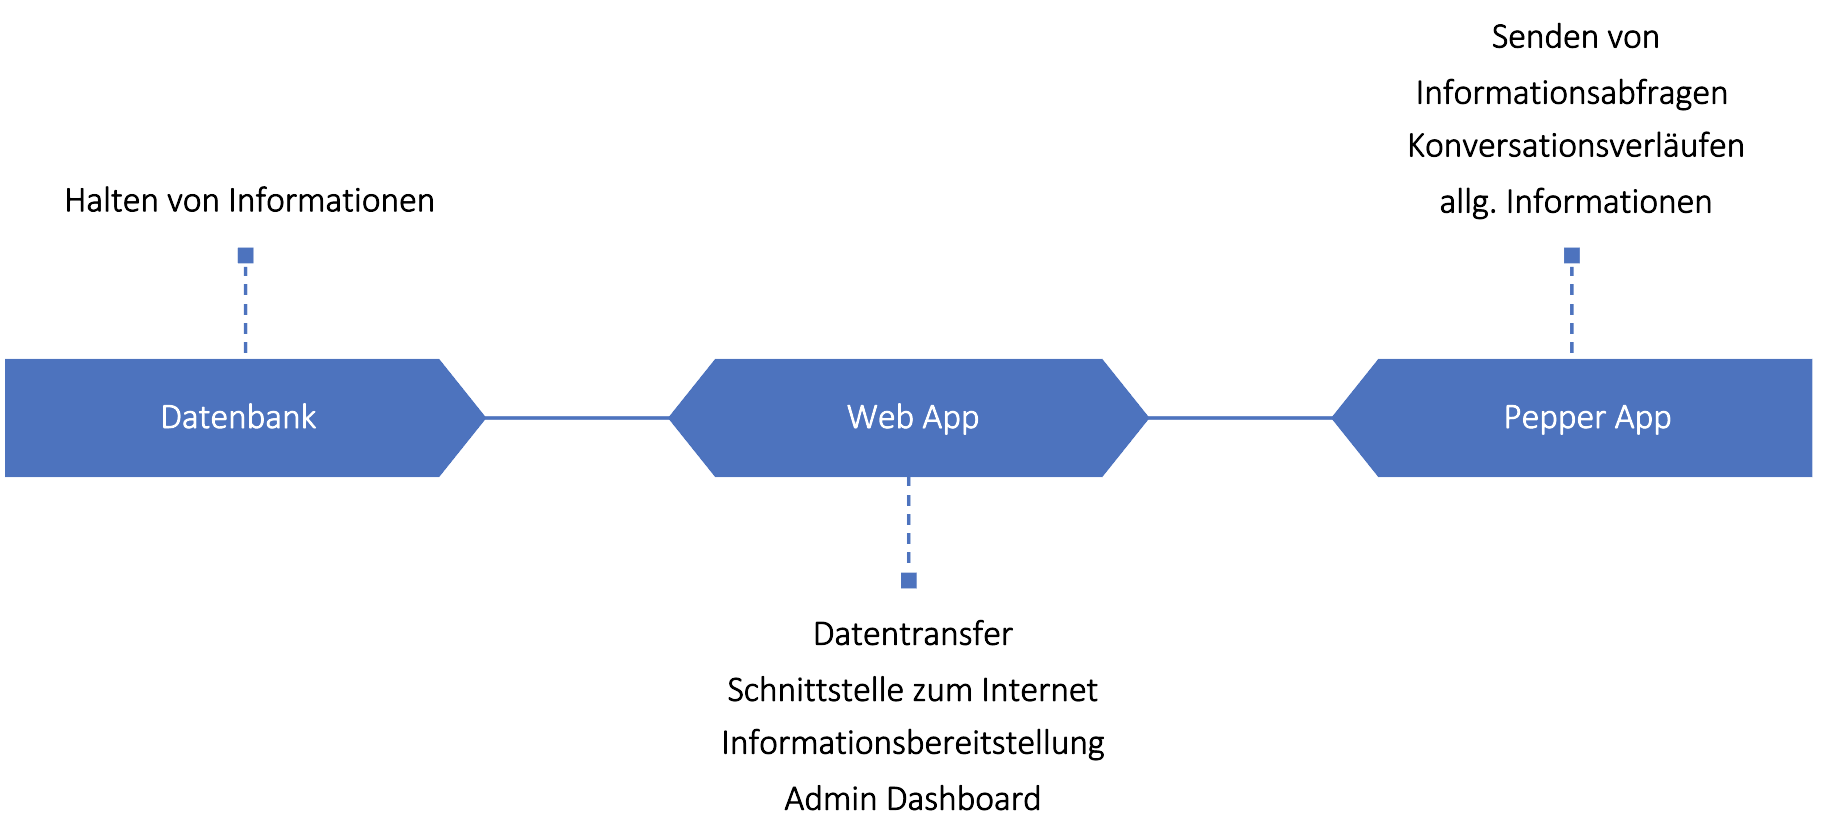
\includegraphics[width=\textwidth]{Figures/NodeChapter/integration.png}
    \caption{Zusammenhang: Pepper App und Backend}
    \label{fig:integration}
    \centering
\end{figure}

Bei der Implementierung der Stundenpläne, werden verschiedene Anfragen an die Hochschulserver geschickt und ausgewertet, jedoch ist auch dies in Java nicht wirklich entwicklerfreundlich. Daher sind wir auf die Idee gekommen, einen Webserver aufzusetzen, den Pepper kontaktieren kann, um weiterführende Informationen zu erhalten.

Genau hier war es uns von Vorteil, Erfahrungen mit Node, Datenbanken und API's gesammelt zu haben. Daher ist es ein leichtes Unterfangen gewesen, einen Express Webserver mit Hilfe der Laufzeitumgebung Node aufzusetzen, auf welchem wir vielfältige Möglichkeiten zur Implementierung von komplexen Vorgängen haben.

So hat es sich ergeben, dass wir nicht nur eine Anwendung für Pepper entwickelt haben, sondern einen zweiten Schwerpunkt, welcher sich auf das Sammeln und Auswerten von Daten konzentriert, definiert haben. Diese Daten sollen natürlich von Pepper über unsere Anwendung gesammelt werden.

Das Repository dieser Webanwendung ist öffentlich und unter folgender Adresse erreichbar: \href{https://github.com/ProjectPepperHSB/NodeJS\_Server4Pepper}{https://github.com/ProjectPepperHSB/NodeJS\_Server4Pepper}. Sollte dieser Link nicht mehr funktionieren, kann sich an die Hochschule gewandt werden, denn auch dort wird unser Quellcode hitnerlegt sein.\\

\section{Überblick: Webanwendung}
\label{sec:nodechapter-ueberblick}
\lhead{\nodechapter \emph{Node - Express Webanwendung: Überblick}}
Bevor wir im Folgenden auf die Implementierung und Spezifikationen unserer Webanwendung eingehen, wollen wir hier kurz die Hauptfunktionalitäten, welche wir in drei Kategorien aufgeteilt haben, aufzeigen.\\

\begin{figure}[H]
    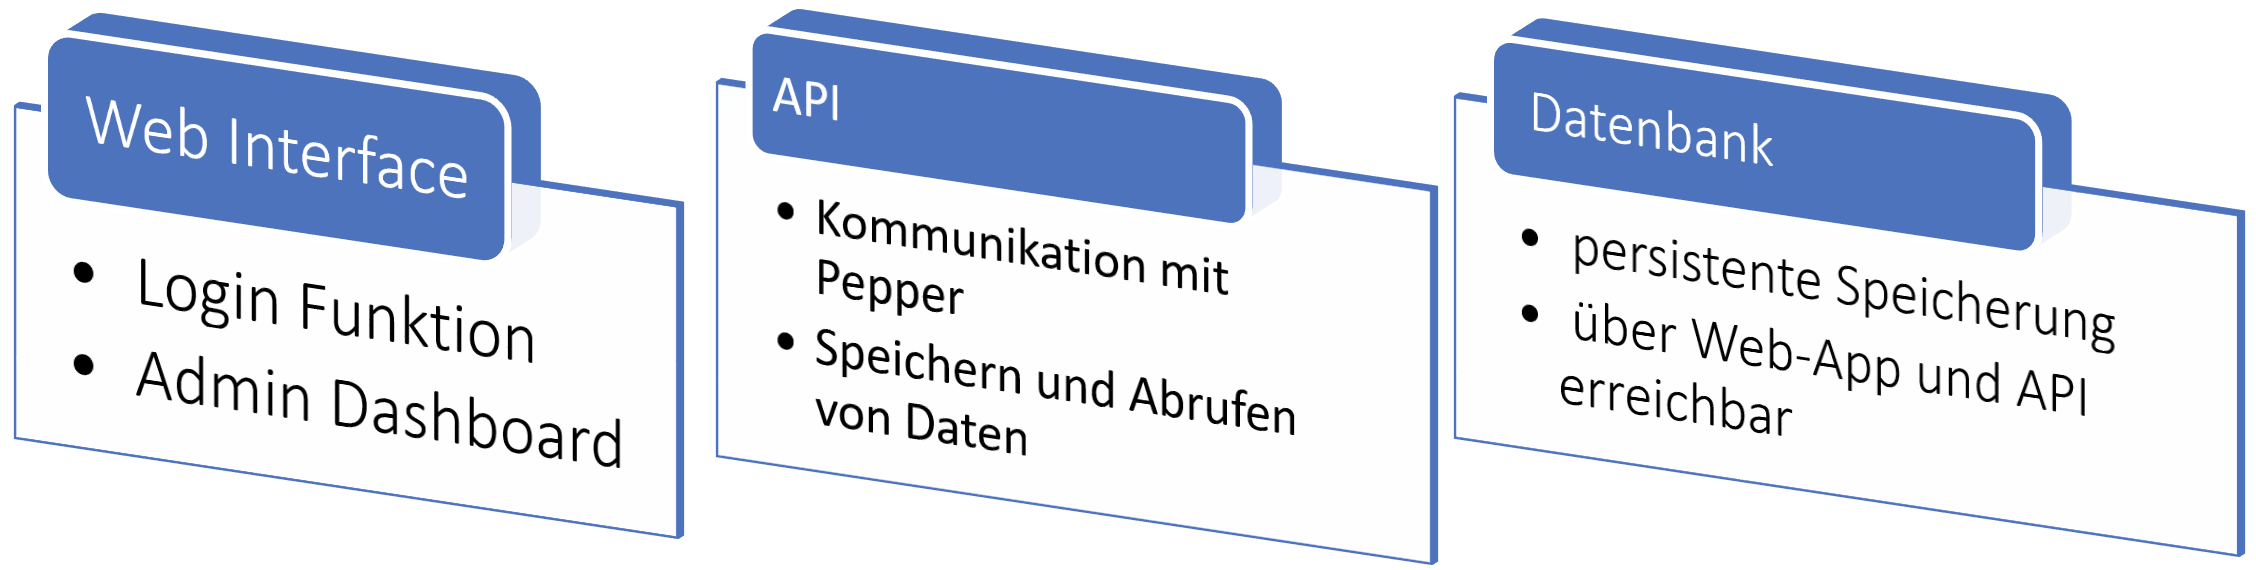
\includegraphics[width=\textwidth]{Figures/NodeChapter/WebAppComponents.png}
    \caption{Komponenten der Webanwendung}
    \label{fig:webappcomponents}
    \centering
\end{figure}

Diese Webanwendung, sowie die dazugehörige Datebank laufen derzeit auf dem Hochschulserver Hopper, in einem abgeschirmten Docker-Kontainer, welcher einem Benutzer mit Namen ``hbv-kms'' gehört. Dies ist ein Benutzer, auf welchen wir gemeinsam als Team zugreifen können. Da die Anwendung über den HTTP Port des Dockers läuft, findet sich der Pfad \verb|docker-hbv-kms-http| in allen Endpunkten dieser Webanwendung wieder.

Diese Anwendung ist jedoch auch auf fast jedem lokalen Rechner ausführbar, sofern eine funktionsfähige MySQL Instanz aktiv ist (vgl. Abschnitt \ref{sec:nodechapter-implementation}).

\subsection{Web Interface}
\label{sec:nodechapter-web-interface}
Das Web Interface dient dazu, den Entwicklern und Betreibern der Webanwendung, Informationen über die gesammelten Daten aufzuzeigen. Da wir es für sinnvoll halten, nicht jedem den kompletten Zugriff auf die gesammelten Daten zu gewähren, haben wir uns dazu entschieden, nur einen Benutzer in unserer Webanwendung anzulegen, welcher Zugriff auf das Admin Dashboard hat. Somit sparen wir uns die Implementierungen zur Registration und Verwaltung von Nutzern (mehr in Abschnitt \ref{sec:nodechapter-implementation}).\\


\begin{figure}[H]
    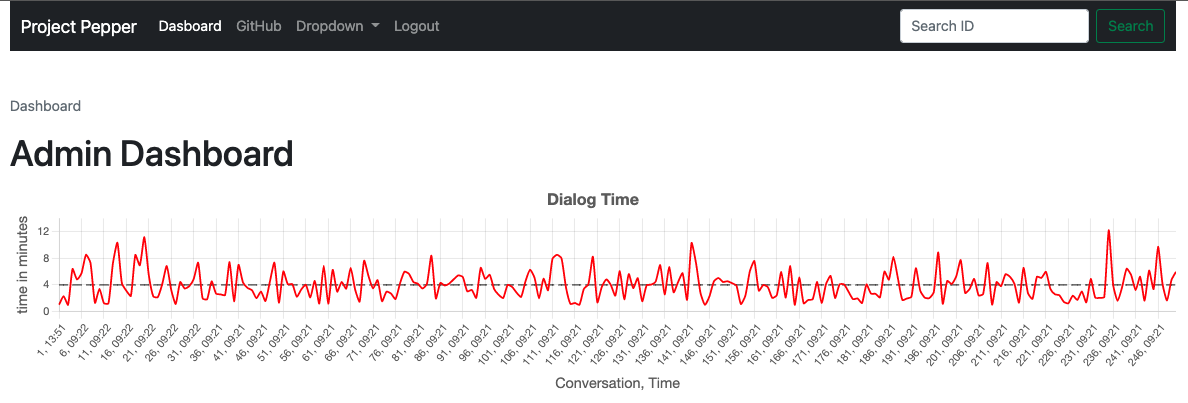
\includegraphics[width=\textwidth]{Figures/NodeChapter/adminDashboard1.png}
    \caption{Webansicht des Admin Dashboards Teil 1}
    \label{fig:admindashboard1}
    \centering
\end{figure}

(Abb. \ref{fig:admindashboard1}) Sofern sich ein Administrator angemeldet hat, gelangt er in die Ansicht des Admin Dashboards. Dieses besteht aus mehreren Komponenten. Zu sehen ist, dass sich am oberen Bereich der Abbildung eine Menüleiste befindet. Diese Beinhaltet eine Verlinkung zu unseren öffentlichen GitHub Repositories, sowie weitere Dropdowns, welche bisher noch keine Funktionen besitzen. Dies ist je nach Anwendungsfall und Einsatzgebiet individuell erweiterbar. Über die Suchleiste kann nach speziellen Identifikationsnummern einzelner Konversationen und Datenreihen gesucht werden. (vgl. Abschnitt \ref{sec:routes-dashboard-detail} f.)

Des Weiteren ist ein Liniendiagramm abgebildet. Dies zeigt die Dauer der letzten 250 Konversationen, welche von Pepper geführt und anschließend über unserer Webanwendung in die Datenbank gespeichert wurden. Dieses Diagramm ist jedoch nicht aussagekräftig, da wir zur Füllung unserer Datenbank, Skripte zur randomisierten Generierung von Konversationen erstellt und ausgeführt haben (vgl. Abschnitt \ref{sec:dummy-data}).

Wir liefern immer nur die letzen 250 Konversationen aus, da Pepper gar nicht so viele Konversationen führen wird, da diese auch eine gewisse Zeit in Anspruch nehmen. Somit ist es nur sinnvoll, sich die letzen 250 anzeigen zu lassen, um einen aktuellen Überblick über die vergangenen Interaktionen zu erhalten. Über die Suchleiste kann dennoch jede Konversation gefunden werden.\\


\begin{figure}[H]
    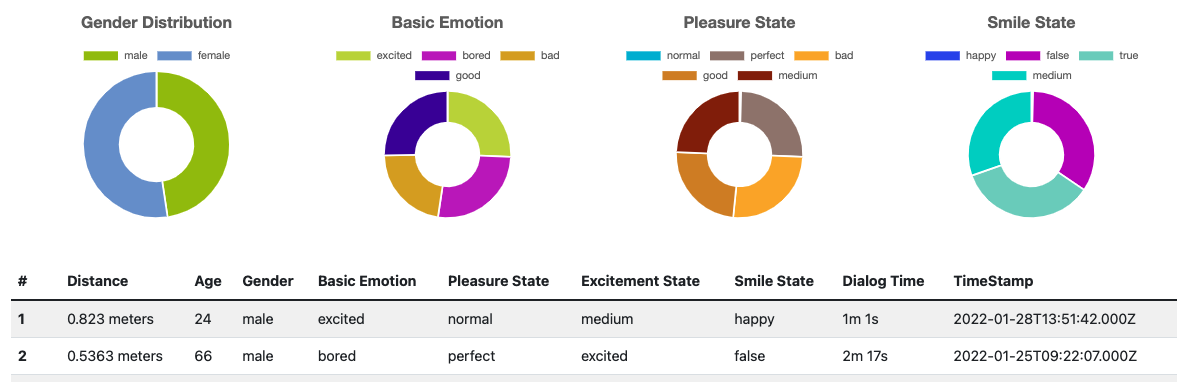
\includegraphics[width=\textwidth]{Figures/NodeChapter/adminDashboard2.png}
    \caption{Webansicht des Admin Dashboards Teil 2}
    \label{fig:admindashboard2}
    \centering
\end{figure}

Zusätzlich zur Darstellung der Konversationsverläufe haben wir uns entschieden, weitere interessante Informationen zu den zur Grunde liegenden Gesprächen visuell hervorzuheben. Somit ist es möglich, sich einen schnellen Überblick
über die letzen Interaktionen mit Pepper zu verschaffen.

(Abb. \ref{fig:admindashboard2}) Sprechen mehr männliche oder weibliche Personen
mit Pepper? Wie ist die Stimmung unserer Akteure und wie verhalten sie sich? Wird gelacht oder sind sie gelangweilt? Diese Informationen können anhand der Donut-Diagramme abgelesen und interpretiert werden. So hat man beispielsweise Auskunft darüber, ob ein neues Update bei den Kunden und Anwendern gut ankommt, oder ob man nicht doch noch etwas ausbessern sollte. Zudem ist auf unseren Anwendungsfall Hochschule bezogen, auch nachvollziehbar, wie die allgemeine Stimmung der Studenten und Interessierten ist.

Unterhalb den Diagrammen beginnt eine Tabelle, welche die ausgewerteten Datenreihen beinhaltet. Jede dieser Reihen führt per Klick auf eine Detailansicht der jeweiligen Konversation und bietet somit einen genaueren Einblick in das geführte
Gespärch.

\begin{figure}[H]
    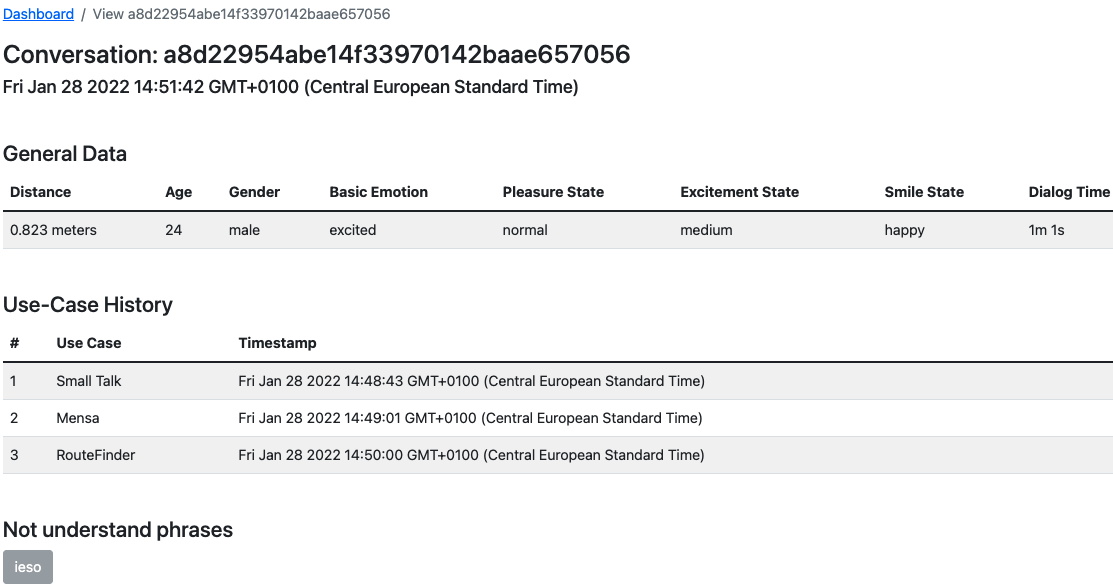
\includegraphics[width=\textwidth]{Figures/NodeChapter/webappdetail.png}
    \caption{Ansicht der Informationen einer Konversation}
    \label{fig:webappdetail}
    \centering
\end{figure}

(Abb. \ref{fig:webappdetail}) Jeder Konversation, die Pepper führt, wird eine Identifikationsnummer zugewisen. Dies ermöglicht die dynamische Zuordnung von Inhalten zu einem bestimmten Gespräch. Somit ist es möglich, Einsicht in die allgemeinen Informationen, wie dem Alter und Geschlecht des Gespärchspartners, zu erhalten. Auch Informationen über verwendete Anwendungsfälle und deren chronologischer Reihenfolge sind abrufbar. Auch Phrasen, welche Pepper nicht verstanden hat, sei es aufgrund von Akzenten oder falscher Aussprache, werden der Konversation zugewiesen.

Dies alles ermöglicht es uns und dem Anwender der Software, mehr über seine Kunden und Anwender zu erfahren - oder auf die Hochschule bezogen: Die Stimmung der Studenten, sowie des Personals und Interessierten kann erfasst werden.

Alle Endpunkte unserer Webanwendung, die für das Admin Dashboard benötigt werden, setzen voraus, dass der Benutzer als Admin angemeldet ist und ein gültiges JSON Web Token in seinem Cookie besitzt.\\


\subsection{API}
\label{sec:nodechapter-api}
Die Kommunikation mit unserer Webanwendung verläuft nicht nur über das Web Interface, sondern über verschiedene Endpunkte, auch Routes genannt. Über diese können je nach Grad der Authentifizierung verschiedene Inhalte gesendet und empfangen werden.

Um hier nicht zu viele Informationen aus den Bereichen der Endpunkte (Abschnitt \ref{sec:nodechapter-implementation-routes}) und Implementierung (Abschnitt \ref{sec:nodechapter-implementation}) vorweg zu nehmen, wollen wir es bei der Erwähnug und Beschreibung der wichtigsten Endpunkte belassen.

\begin{itemize}
    \item /docker-hbv-kms-http/fileserver
    \item /docker-hbv-kms-http/api/v1/sql
    \item /docker-hbv-kms-http/api/save$\left[context\right]$Data
\end{itemize}

(vgl Abschnitt \ref{sec:api-fileserver}) Wir haben aufgrund der Struktur unserer Serverkonfiguration zunächst Schwierigkeiten gehabt, statische Dateien über HTTP auszuliefern, da sich die Pfade zwischen der lokal laufenden Instanz von denen der auf dem Hopper laufenden unterscheiden. Daher haben wir einen Endpunkt \verb|/docker-hbv-kms-http/fileserver| erstellt, welcher uns dynamisch die gewünschte Datei Pfadunabhängig ausliefern kann. Hierbei wurde auch berücksichtigt, dass nur bestimmte Dateien ausgeliefert werden können. Es wäre fatal, wenn man dies nicht beachtet und in einer Produktivumgebung alle Dateien des Servers, einschließlich der Zertifikate ausliefern würde.

(vgl. Abschnitt \ref{sec:api-sql-query}) Der Endpunkt \verb|/docker-hbv-kms-http/api/v1/sql| ist die Schnittstelle über welche man extern auf Daten in der
Datenbank zugreifen kann. Hier ist es erforderlich, authentifiziert zu sein.
Dafür muss ein Auth-Token bei jeder Abfrage übermittelt werden, welches mit dem Token, das in unserer Webanwendung hinterlegt ist, verglichen wird. Um das Problem des öffentlichen Einsehens unseres Tokens durch Github zu vermeiden, arbeiten wir mit \verb|.env| Dateien, welche während der Initialisierung der Webanwendung geladen wird. Diese \verb|.env| Datei ist nicht auf Github, jedoch existiert eine Beispieldatei mit namen \verb|.example.env|, welche das Format und die
nötigen Felder vorgibt.

Der letzte oben aufgeführte Endpunkt, steht symbolisch für eine Reihe von Endpunkten, welche für die Speicherung verschiedener Informationen, die Pepper während seiner Gespräche sammelt und an unserern Server übermittelt, verantwortlich ist. Diese Endpunkte sind sowohl über GET, als auch über POST Anfragen ansprechbar und nehmen verschiedene Parameter entgegen. Bisher muss man sich für diese Endpunkte nicht authentifizieren, das heißt, dass jeder in unsere Tabellen schreiben kann, sofern er die richtigen Parameter kennt. Wir haben überlegt dies zu umgehen, indem wir Pepper ebenfalls ein Token generieren lassen, welches als zur Authentifizierung mit der Webanwendung verwendet wird, jedoch würde dies das Problem nur verlagern, da unser gesamter Quellcode öffentlich einsehbar ist. Dies kann, soweit wir wissen, nicht über Umgebungsvariablen in Andriod Studio umgangen werden.

Es gibt natürlich noch viele weitere Endpunkte in unserer Webanwendung, wie zum Beispiel den, zur Abfrage von Stunden- oder Mensaplänen. Dieser bekommt Parameter übergeben, woraufhin mit Hilfe verschiedener Methoden die gewünschten Informationen bereitgestellt werden (vgl. Abschnitt \ref{sec:nodechapter-implementation-routes}).\\

\subsection{Datenbank}
\label{sec:nodechapter-database}
Um die Informationen, welche unser Pepper während seiner Gespräche sammelt auch persistent speichern zu könenn, haben wir uns dazu entschieden, eine MySQL Datenbank zu integrieren. Zunächst haben wir es als fortschrittlicher gehalten, MongoDB zu verwenden, da dies eine JSON-Objekt basierte Speicherung von Daten ermöglicht und durch seine skalierbare und einfache Integration in Expres und JavaScript vielfältige Möglichkeiten bietet.

MongoDB ist jedoch nicht auf dem Hochschulserver installiert und da wir durch verschiedene Kurse schon sehr gute Kenntnisse und Erfahrungen mit MySQL gesammelt haben, war es dann doch nicht so schlimm, auf MongoDB zu verzichten.

Die von der Webanwendung verwendete Datenbank läuft in dem zuvor erwähnten Docker-Kontainer des geteilten Benutzers.

Weitere Informationen und Spezifikationen sind der Tabelle im Abschnitt \ref{sec:nodechapter-versions} zu entnehmen.

% -------- -------- -------- -------- -------- -------- -------- -------- -------- -------- -------- 
% -------- -------- -------- -------- -------- -------- -------- -------- -------- -------- -------- 
% -------- -------- -------- -------- -------- -------- -------- -------- -------- -------- -------- 
% -------- -------- -------- -------- -------- -------- -------- -------- -------- -------- -------- 
% -------- -------- -------- -------- -------- -------- -------- -------- -------- -------- -------- 
% -------- -------- -------- -------- -------- -------- -------- -------- -------- -------- -------- 

\newpage
\section{Endpunkte und Responses der Webanwendung}
\label{sec:nodechapter-implementation-routes}
\lhead{\nodechapter \emph{Node - Express Webanwendung: Endpunkte und Responses}}
Unsere Webanwendung ist über viele Endpunkte ansprechbar. Nachfolgend sind diese in zwei Gruppen Aufgeteilt. Endpunkte, welche für das Admin Dashboard benötigt werden, sowie als Resultat eine HTML Seite rendern, sind unter dem Abschnitt \ref{sec:routes} zu finden. Alle weiteren Endpunkte, welche zumeist nur Daten entgegen nehmen oder Informationen in Form von JSON zurück geben, sind in Abschnitt \ref{sec:api-routes} aufgelistet.

\subsection{Web Interface Endpunkte / Routes}
\label{sec:routes}
\dotfill
\subsubsection{Startseite}
\label{sec:routes-start}
\textbf{Beschreibung:} Liefert die Startseite der Webanwendung wieder. Auf dieser ist nur der Titel der Anwendung, sowie einen Button, der zur Login Seite führt (siehe \ref{sec:routes-login}).

\textbf{Methode:} GET

\textbf{Endpunkt:} /docker-hbv-kms-http/

\textbf{Parameter:}
keine

\dotfill

\subsubsection{Dashboard}
\label{sec:routes-dashboard}
\textbf{Beschreibung:} Liefert einem angemeldetem Admin die Ansicht des Dashboards (vgl. Abb. \ref{fig:admindashboard1} und \ref{fig:admindashboard2}).

\textbf{Methode:} GET

\textbf{Endpunkt:} /docker-hbv-kms-http/dashboard

\textbf{Parameter:}
keine

\dotfill

\subsubsection{Dashboard: Detailansicht}
\label{sec:routes-dashboard-detail}
\textbf{Beschreibung:} Dient der visuellen Übermittlung der Detailansicht einer Konversation (vgl. Abb. \ref{fig:webappdetail}). Dies ist nur über den Browser erreichbar, sofern ein gültiges JSON Web Token im Cookie hinterlegt ist.

\textbf{Methode:} GET

\textbf{Endpunkt:} /docker-hbv-kms-http/dashboard/view

\textbf{Parameter:}
\begin{table}[H]
    \label{table:/docker-hbv-kms-http/dashboard/view}
    \setlength{\tabcolsep}{3pt}
    \begin{tabular}{p{100pt}p{80pt}p{200pt}}
        \toprule
        Param            & Typ    & Beschreibung                        \\                                                             \\
        \midrule
        conversation\_id & String & ID der zu abzurufenden Konversation \\
        \bottomrule
    \end{tabular}
\end{table}
\dotfill

\subsubsection{Dashboard: Datenabfrage}
\label{sec:routes-dashboard-query}
\textbf{Beschreibung:} Dieser Endpunkt dient der Abfrage von \textit{n} Datenreihen, welche auf dem Admin Dashboard dargestellt werden. Dies wird für die Tabelle, sowie für die dortigen Visualisierungen verwendet.

\textbf{Methode:} GET

\textbf{Endpunkt:} /docker-hbv-kms-http/api/v1/getData

\textbf{Parameter:}
\begin{table}[H]
    \label{table:/docker-hbv-kms-http/api/v1/getData}
    \setlength{\tabcolsep}{3pt}
    \begin{tabular}{p{100pt}p{80pt}p{200pt}}
        \toprule
        Param & Typ    & Beschreibung                        \\
        \midrule
        n     & String & Anzahl der abzurufenden Datenreihen \\
        \bottomrule
    \end{tabular}
\end{table}
\dotfill

\subsubsection{Login}
\label{sec:routes-login}
\textbf{Beschreibung:} Liefert bei einer GET Anfrage die Login Seite aus. Der POST Endpunkt wird nach Abschicken des Login-Forumulars angesprochen, validiert den Login und leitet den Client bei Erfolg an das Dashboard weiter. Gleichzeitig wird das JSON Web Token im Cookie des Clients hinterlegt.

\textbf{Methode:} GET, POST

\textbf{Endpunkt:} /docker-hbv-kms-http/dashboard/login

\textbf{Parameter GET:} keine

\textbf{Parameter POST:}
\begin{table}[H]
    \label{table:/docker-hbv-kms-http/login}
    \setlength{\tabcolsep}{3pt}
    \begin{tabular}{p{100pt}p{80pt}p{200pt}}
        \toprule
        Param           & Typ    & Beschreibung \\                                                             \\
        \midrule
        username\_input & String & Benutzername \\
        password\_input & String & Passwort     \\
        \bottomrule
    \end{tabular}
\end{table}
\dotfill

\subsubsection{Logout}
\label{sec:routes-logout}
\textbf{Beschreibung:} Löscht das JSON Web Token aus dem Cookie des Benutzers und meldet ihn somit ab. Anschließend wird nach /docker-hbv-kms-http/ weiter geleitet (vgl. Abschnitt \ref{sec:routes-start}).

\textbf{Methode:} GET

\textbf{Endpunkt:} /docker-hbv-kms-http/dashboard/logout

\textbf{Parameter:} keine

\dotfill






\subsection{API Endpunkte / Routes}
\label{sec:api-routes}
Alle Endpunkte, welche nicht über ein GUI angesprochen werden, sind mit \verb|api| in der URI hiterglegt. Anschließend ist die Versionsnummer des Endpunktes anzugeben. Bisher gibt es nur die Version 1.

\subsubsection{Speicherung von Emotionsdaten}
\label{sec:api-saveEmotionData}
\textbf{Beschreibung:} Dieser Endpunkt dient der Speicherung verschiedener Daten, welche sich im Verlauf einer Konversation mit Pepper ergeben.

\textbf{Methode:} GET

\textbf{Endpunkt:} /docker-hbv-kms-http/api/v1/saveEmotionData

\begin{table}[H]
    \label{table:/docker-hbv-kms-http/api/v1/saveEmotionData}
    \setlength{\tabcolsep}{3pt}
    \begin{tabular}{p{100pt}p{80pt}p{200pt}}
        \toprule
        Param             & Typ            & Beschreibung                                            \\
        \midrule
        identifier        & String         & Identifikationsnummer der Konversation                  \\
        distance          & String / Float & [optional] Distanz zwischen Pepper und dem Sprecher     \\
        age               & String / Float & [optional] Alter des Sprechers                          \\
        gender            & String         & [optional] Geschlecht des Sprechers                     \\
        basic\_emotion    & String         & [optional] Generelle Stimmung des Sprechers             \\
        pleasure\_state   & String         & [optional] Motivation des Sprechers                     \\
        excitement\_state & String         & [optional] Begeisterung des Sprechers                   \\
        smile\_state      & String         & [optional] Einschätzung der Glücklichkeit des Sprechers \\
        dialog\_time      & String / Float & [optional] Zeit des Gespräches                          \\
        \bottomrule
    \end{tabular}
\end{table}

\dotfill

\subsubsection{Speicherung des verwendeten Anwendungsfalles}
\label{sec:api-saveUseCaseData}
\textbf{Beschreibung:} Realisierung der Speicherung der in einer Konversation verwendeten Anwendungsfälle.

\textbf{Methode:} GET

\textbf{Endpunkt:} /docker-hbv-kms-http/api/v1/saveUseCaseData

\begin{table}[H]
    \label{table:/docker-hbv-kms-http/api/v1/saveUseCaseData}
    \setlength{\tabcolsep}{3pt}
    \begin{tabular}{p{100pt}p{80pt}p{200pt}}
        \toprule
        Param      & Typ    & Beschreibung                           \\
        \midrule
        identifier & String & Identifikationsnummer der Konversation \\
        use\_case  & String & Name des Use-Cases                     \\
        \bottomrule
    \end{tabular}
\end{table}

\dotfill

\subsubsection{Speicherung von nicht verstandenen Phrasen}
\label{sec:api-saveNotUnderstandPhrases}
\textbf{Beschreibung:} Realisierung der Speicherung der von Pepper nicht verstandenen Wörter und Phrasen.

\textbf{Methode:} GET

\textbf{Endpunkt:} /docker-hbv-kms-http/api/v1/saveNotUnderstandPhrases

\begin{table}[H]
    \label{table:/docker-hbv-kms-http/api/v1/saveNotUnderstandPhrases}
    \setlength{\tabcolsep}{3pt}
    \begin{tabular}{p{100pt}p{80pt}p{200pt}}
        \toprule
        Param      & Typ    & Beschreibung                           \\
        \midrule
        identifier & String & Identifikationsnummer der Konversation \\
        phrase     & String & Nicht verstandene Phrase               \\
        \bottomrule
    \end{tabular}
\end{table}

\dotfill

\subsubsection{Speicherung von zusätzlichen Daten}
\label{sec:api-saveAttributeData}
\textbf{Beschreibung:} Dieser Endpunkt ermöglicht die Speicherung von weiteren Variablen und nicht vordefinierten Informationen.

\textbf{Methode:} POST

\textbf{Endpunkt:} /docker-hbv-kms-http/api/v1/saveAttributeData

\begin{table}[H]
    \label{table:/docker-hbv-kms-http/api/v1/saveAttributeData}
    \setlength{\tabcolsep}{3pt}
    \begin{tabular}{p{100pt}p{80pt}p{200pt}}
        \toprule
        Param      & Typ           & Beschreibung                           \\
        \midrule
        identifier & String        & Identifikationsnummer der Konversation \\
        data       & String / JSON & variable Daten der Konversation        \\
        \bottomrule
    \end{tabular}
\end{table}
\dotfill



\subsubsection{Abfrage von Daten aus der DB mittels SQL Query String}
\label{sec:api-sql-query}
\textbf{Beschreibung:} Endpunkt zur Interaktion mit der Datenbank. Ein API-Token wird benötigt. SQL Befehle können übermittelt werden. Aus Sicherheitsgründen werden Anfragen, welche folgende Wörter beinhalen, abgelehnt: \verb|CREATE|, \verb|DROP|, \verb|DELETE|, \verb|SHOW|, \verb|USERS|, \verb|INSERT|, \verb|INTO|. Dies gilt für Groß-und Kleinschreibung. Bei erfolgreicher Abfrage wird das Ergebnis des SQL-Statements als JSON zurückgeliefert.

\textbf{Methode:} POST

\textbf{Endpunkt:} /docker-hbv-kms-http/api/v1/sql

\textbf{Parameter:}
\begin{table}[H]
    \label{table:/docker-hbv-kms-http/api/v1/sql}
    \setlength{\tabcolsep}{3pt}
    \begin{tabular}{p{100pt}p{80pt}p{200pt}}
        \toprule
        Param      & Typ    & Beschreibung               \\
        \midrule
        auth\_key  & String & API-Token                  \\
        subject    & String & [optional] Art der Abfrage \\
        sql\_query & String & Auszuführender SQL Befehl  \\
        \bottomrule
    \end{tabular}
\end{table}
\dotfill

\subsubsection{Abfrage des Stundenplans}
\label{sec:api-timetable}
\textbf{Beschreibung:} Dient der Abfrage von Stundenplänen eines bestimmten Studiengangs. Bei erfolgreicher Abfrage wird ein JSON Objekt, oder einen HTML String zurückgegeben.

\textbf{Methode:} GET

\textbf{Endpunkt:} /docker-hbv-kms-http/api/v1/timetable

\textbf{Parameter:}
\begin{table}[H]
    \label{table:/docker-hbv-kms-http/api/v1/timetable}
    \setlength{\tabcolsep}{3pt}
    \begin{tabular}{p{100pt}p{80pt}p{200pt}}
        \toprule
        Param    & Typ              & Beschreibung                                        \\
        \midrule
        course   & String           & Studiengang (Kürzel wie: ``WI'', ``BWL'' etc.)      \\
        kw       & String / Integer & [optional] Kalenderwoche                            \\
        semester & String / Integer & [optional] Semester                                 \\
        htmlOnly & Boolean          & [optional] HTML oder JSON Response (Default: false) \\
        \bottomrule
    \end{tabular}
\end{table}
\dotfill


\subsubsection{Abfrage des Mensaplans als JSON}
\label{sec:api-mensa-json}
\textbf{Beschreibung:} Liefert den Mensaplan für die aktuelle Woche als JSON Objekt zurück.

\textbf{Methode:} GET

\textbf{Endpunkt:} /docker-hbv-kms-http/api/v1/mensadata

\textbf{Parameter:} keine

\dotfill

\subsubsection{Abfrage des Mensaplans als Bild}
\label{sec:api-mensa-img}
\textbf{Beschreibung:} Liefert den Mensaplan fur die aktuelle Woche als Bild zurück.

\textbf{Methode:} GET

\textbf{Endpunkt:} /docker-hbv-kms-http/api/v1/mensadata/img

\textbf{Parameter:} keine

\dotfill

\subsubsection{File Server}
\label{sec:api-fileserver}
\textbf{Beschreibung:} Dieser Endpunkt wird verwendet, Skripte und Stylesheets dynamisch aus dem \verb|static| Verzeichnis
abzurufen.

\textbf{Methode:} GET

\textbf{Endpunkt:} /docker-hbv-kms-http/fileserver

\textbf{Parameter:}
\begin{table}[H]
    \label{table:/docker-hbv-kms-http/fileserver}
    \setlength{\tabcolsep}{3pt}
    \begin{tabular}{p{100pt}p{80pt}p{200pt}}
        \toprule
        Param & Typ    & Beschreibung                 \\
        \midrule
        name  & String & Name der angeforderten Datei \\
        \bottomrule
    \end{tabular}
\end{table}
\dotfill


\subsubsection{Abfrage des Kurspreises einer Kryptowährung}
\label{sec:api-crypto}
\textbf{Beschreibung:} Dieser Endpunkt kann einem den Kurspreis und weitere relevante Informationen zu einem Kryptowährungs-Handelspaar zurückliefern.

\textbf{Methode:} GET

\textbf{Endpunkt:} /docker-hbv-kms-http/api/v1/crypto

\textbf{Parameter:}
\begin{table}[H]
    \label{table:/docker-hbv-kms-http/api/v1/crypto}
    \setlength{\tabcolsep}{3pt}
    \begin{tabular}{p{100pt}p{80pt}p{200pt}}
        \toprule
        Param   & Typ    & Beschreibung                                  \\
        \midrule
        subject & String & Anforderung (nur ``price'' ist implementiert) \\
        symbol  & String & Symbol (Bsp.: ``BTC-USDT'')                   \\
        \bottomrule
    \end{tabular}
\end{table}
\dotfill

\subsubsection{Abfrage der IP-Adresse des Clients}
\label{sec:api-client-ip}
\textbf{Beschreibung:} Liefert die IP Adresse des Clients zurück.

\textbf{Methode:} GET

\textbf{Endpunkt:} /docker-hbv-kms-http/api/v1/ip

\textbf{Parameter:} keine

\dotfill


\subsection{Responses und Status Codes}
\label{sec:nodechapter-implementation-responses}
Alle An- und Abfragen an unsere Webanwendung liefern verschiedene Antworten / Responses zurück. In der nachfolgenden Tabelle sind die Geläufigsten aufgelistet. Da gewisse Error-Handling-Mechanismen automatisch eine entsprecheende Antwort liefern, kann es zu abweichenden Beschreibungen und weiteren Status Codes kommen.
\begin{table}[H]
    \caption{Status Codes und deren Bedeutung }
    \label{tab:responsecodes}
    \setlength{\tabcolsep}{3pt}
    \begin{tabular}{p{100pt}p{280pt}}
        % \toprule
        Status Code & Bedeutung             \\
        \midrule
        200         & OK                    \\
        400         & Invalid Parameter     \\
        401         & Unauthorized          \\
        404         & Not Found             \\
        500         & Internal Server Error \\
        \bottomrule
    \end{tabular}
\end{table}

% -------- -------- -------- -------- -------- -------- -------- -------- -------- -------- -------- 
% -------- -------- -------- -------- -------- -------- -------- -------- -------- -------- -------- 
% -------- -------- -------- -------- -------- -------- -------- -------- -------- -------- -------- 
% -------- -------- -------- -------- -------- -------- -------- -------- -------- -------- -------- 
% -------- -------- -------- -------- -------- -------- -------- -------- -------- -------- -------- 
% -------- -------- -------- -------- -------- -------- -------- -------- -------- -------- -------- 

\newpage
\section{Implementierung}
\label{sec:nodechapter-implementation}
\lhead{\nodechapter \emph{Node - Express Webanwendung: Implementierung}}
Bei unserer Web App handelt es sich um eine Anwendung, welche mit dem Framework Express für die Laufzeitumgebung Node entwickelt wurde. Express zeichnet sich durch die simple Konfiguration, sowie einfache Implementierung verschiedenster Funktionalitäten aus. Express wird meist für Backendanwendungen verwendet, wir benutzen es jedoch auch, um serverseitiges Rendering zu realisieren. Dies bedeutet, dass Ansichten / Views, welche an den Client ausgeliefert werden, zuvor auf dem Server generiert worden sind.\\

\subsection{Allgemein}
Von außen ist unsere Anwendung über die URL
\href{https://informatik.hs-bremerhaven.de/docker-hbv-kms-http}{https://informatik.hs-bremerhaven.de/docker-hbv-kms-http} erreichbar. Sollte sie lokal ausgeführt werden, muss die Domain auf Localhost geändert werden - hier ist dann auch die Angabe des Ports nötig (mehr in Abschnitt \ref{sec:nodechapter-installation}).

Unsere Anwendung besitzt jedoch nicht all zu viele Views, bis auf das zuvor gezeigte Admin Dashboard (vgl. Abschnitt \ref{sec:routes-dashboard}), sowie die Detailansicht der einzelnen Daten der Konversationen (vgl. Abschnitt \ref{sec:routes-dashboard-detail}). Darüber hinaus gibt es nur die Startseite und die Login-View. Diese Login-View ist über den Endpunkt \verb|/docker-hbv-kms-http/login| (vgl. Abschnitt \ref{sec:routes-login}) erreichbar und beinhaltet nur ein Formular zur Eingabe des Benutzernamens, sowie des dazugehörigen Passwortes.

Abbildung \ref{fig:webhierarchie} zeigt den Inhalt des Root-Verzeichnisses unserer Webanwendung. Im Folgenden wird auf die einzelnen Inhalte eingegangen. \\

\begin{figure}[H]
    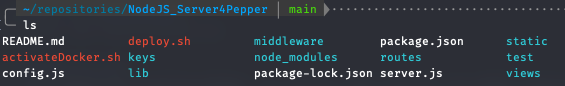
\includegraphics[width=\textwidth]{Figures/NodeChapter/ServerFileStructure.png}
    \caption{Hierarchie des Stammverzeichnisses der Webanwendung}
    \label{fig:webhierarchie}
    \centering
\end{figure}

\subsubsection*{/server.js}
Der Einstiegspunkt unserer Webanwendung ist das Skript \verb|server.js|. Dieses beinhaltet die Einbindung aller benötigten Dateien und Skripte, sowie die Anwendung der in den Konfigurationsdateien festgelegten Einstellungen.

\subsubsection*{/node\_modules, /package-lock.json und /package.json}
Da wir Node als Laufzeitumgebung gewählt haben, ist es uns möglich den Node Package Manager (npm) zur Installation verschiedener Module anzuwenden. Alle installierten Module sind in dem Verzeichnis \verb|node_modules| zu finden. Deren Spezifikationen sind in den Konfigurationsdateien \verb|package.json|, sowie \verb|package-lock.json| festgehalten. \verb|package-lock.json| ist eine automatisch generierte Datei, welche Node verwendet, um Dependencies und Versionen festzuhalten. Aufgrund dieser Konfigurationsdateien ist es nicht nötig, alle im Verzeichnis \verb|node_modules| befindlichen Erweiterungen in das jeweilige GitHub Repository zu laden, denn diese können, nach einer neuen Initialisierung über den Befehl \verb|npm init| anhand der Definitionen in \verb|package-lock.json|, automatisch nachinstalliert werden.

\subsubsection*{/views}
In diesem Verzeichnis befinden sich Templates der Seiten, welche vom Server gerendert und an den Client ausgeliefert werden.

\subsubsection*{/routes}
Der Ordner \verb|routes| beinhaltet die verschiedene Skripte, welche die  nterschiedlichen Endpunkte unserer Webanwendung definieren. Innerhalb dieser Skritpe werden auch die Ansichten aus dem \verb|views|-Verzeichnis gerendert und an den Client geschickt. Hier sind alle in Abschnitt \ref{sec:nodechapter-implementation-routes} behandelten Endpunkte definiert. Die jeweiligen Routes implementieren die jeweiligen Funktionalitäten, sind über Requests ansprechbar und interagieren ggf. mit der Datenbank und anderen Services.

\subsubsection*{/static}
Hier befinden sich statische Dateien, dazu gehören Bilder und unabhängige Skripte, sowie Stylesheets. Diese werden über unsere Route \verb|docker-hbv-kms-http/fileserver| ausgeliefert (vgl. Abschnitt \ref{sec:nodechapter-api}).

\subsubsection*{/middleware}
Bei Middlewares handelt es sich um Skripte, welche Abläufe beinhalten, die zwischen anderen Prozessen statt finden. Hierzu gehört bei uns die Authentifizierung von Nutzern, indem das sich dort befindliche Skript \verb|auth.js| eingebunden wird, während ein Nutzer einen beschränkten Endpunkt anspricht. Dies sorgt dafür, dass nur ausgewählte Benutzer bestimmte Endpunkte erfolgreich ansprechen können. Alle anderen bekommen die Mitteilung, dass sie nicht die nötigen Berechtigungen besitzen.

\subsubsection*{/lib}
Im Ordner \verb|lib| (aka Libraries) befinden sich alle von uns für die Webanwendung verwendeten Skripte, für welche wir keine genaue Unterkategorie finden konnten. Hierbei handelt es sich um Skripte, welche Anfragen synchron und asynchron durchführen können, sowie Funktionen zur Generierung und Validierung von Passwörtern und deren Hashes.

\subsubsection*{/keys}
Da wir beschränkte Endpunkte haben und unsere Authentifizierung mittels JSON Web Token im Cookie des Clients realisiert ist, muss unsere Anwendung dieses Token auch auf Richtigkeit überprüfen können. Daher haben wir uns dazu entschieden ein Schlüsselpaar zu generieren, welches für die Ver-und Entschlüsselung der JSON Web Tokens verwendet wird.\\

\subsubsection*{Sonstige Dateien}
\label{sec:node-other-files}
Im Hauptverzeichnis befinden sich weitere Dateien, wie die README.md, welche eine Quick-Start Anleitung bietet, die in dem Repository der Webanwendung dargestellt ist.

Des weiteren befindet sich ein Skript zum Aktivieren des Docker-Kontainers und ein Deploy-Skript, welches für die Aktivierung des Dockers, das Übertragen der Daten in das entsprechende Verzeichnis, sowie für den Start der Webanwendung sorgt.

Im Repository ist auch die Datei \verb|.example.env| zu finden, welche ein Beispiel dafür bietet, wie die \verb|.env| Datei aussehen muss. Diese .env Datei legt Umgebungsvariablen fest und beinhaltet sensible Daten, wie die Informationen zum Login in die Datenbank, sowie den API-Key zur Nutzung der API über externe Programme / Skripte (vgl. Abschnitt \ref{sec:api-sql-query}). Auch die Festlegung des Ports findet dort statt.\\


\subsection{Error-Handling}
\label{sec:nodechapter-error-handling}
Auch das Behandeln und Abwenden von Fehlern gehört zu einer guten Webanwendung dazu. Hierbei haben wir alle Endpunkte damit bedacht, entsprechende Fehlermeldungen bzw. Antworten an den Client zu senden. Tabelle \ref{tab:responsecodes} zeigt unter anderem auch die geläufigsten Fehlermeldungen. Diese werden beispielsweise dann zurückgegeben, wenn ein Nutzer auf einen Bereich zugreift, für welchen er nicht die entsprechende Berechtigung vorwesein kann oder fehlerhafte bzw. ungültigte Informationen an einen Endpunkt sendet. Sollten Pfade angesprochen werden, die nicht verfügbar sind, wird der Status Code 404 zurückgegeben. Dies ist in der Datei \verb|server.js| definiert.

Wir loggen unsere Fehler nicht selbst, da dies in diesem Rahmen etwas zu viel wäre, jedoch benutzen wir den Prozessmanager \verb|pm2|, welcher für uns das Logging übernimmt.\\


\subsection{Versionen und Spezifikationen}
\label{sec:nodechapter-versions}
Unsere Webanwendung basiert auf Node, JavaScript und dem JavaScript Framework Express. Node ist eine Laufzeitumgebung, welche JavaScript außerhalb des Browsers ausführen kann und somit wichtige Prozesse auf dem Server anstatt beim Client ausführt. Node hat einen eigenen Paketmanager, npm (Node Package Manager), mit welchem sich vielfältige Libraries und Frameworks installieren lassen.

Mit \verb|npm| haben wir zum Beispiel den Prozessmanager \verb|pm2| installiert, welcher Prozesse organisiert und bei Abstürzen neu startet. Auch ein Cluster Mode, bei dem Prozesse in mehreren Instanzen laufen können, ist hiermit möglich. Somit ist ein Totalausfall der Anwendung vermeidbar, sofern die Server der Hochschule keine Schwierigkeiten haben.

Es gibt sehr viele weitere Module, welche wir mittels npm installiert haben. Da viele Module von andern Modulen abhängen und npm automatisch die Abhängigen Module mit installiert, wäre es hier nicht sinnvoll, hunderte Module aufzulisten. Deshalb haben wir uns entschieden in folgender Tabelle nur die zwei wichtigsten Module, \verb|pm2| und Express, aufzulisten.

\begin{table}[H]
    \caption{Hard- und Softwarespezifikationen der Webanwendung}
    \label{tab:node-specs}
    \setlength{\tabcolsep}{3pt}
    \begin{tabular}{|p{70pt}|p{120pt}|p{180pt}|}
        \hline
        Software / Modul & Version / Spezifikation                            & Beschreibung                                           \\
        \hline\hline
        Node             & v16.13.1                                           & Laufzeitumgebung                                       \\
        \hline
        npm              & v8.3.2                                             & Paketmanager für Node                                  \\
        \hline
        MySQL            & v15.1 Distrib 10.6.5-MariaDB, for debian-linux-gnu & Datenbank                                              \\
        \hline
        Express          & v4.17.2                                            & JS Framework für Webserver / Webanwendung (Node Modul) \\
        \hline
        pm2              & v5.1.2                                             & Prozessmanager (Node Modul)                            \\
        \hline
        \multicolumn{3}{p{400pt}}{Node Module sind mit Hilfe von npm installiert worden und müssen regelmäßig geupdated werden.}
    \end{tabular}
\end{table}

Unsere Anwendung ist so konzipiert, dass sie auf den Betriebssystemen Ubuntu, macOS12+ und MS Windows 7+ läuft, sofern alle benötigten Pakete, Module, Tools und Sprachen installiert sind.\\

\newpage
\section{Installation und Konfiguration}
\label{sec:nodechapter-installation}
In Abschnitt \ref{sec:node-other-files} haben wir die Datei README.md angesprochen. Diese bietet einen schnellen Überblick über die benötigte Software (Node, npm und MySQL), sowie die Befehle zur Installation aller benöitgten Tools. Im Folgenden werden wir diese Schritte aufzeigen.

\subsection*{Installation}
\label{sec:nodechapter-installation}
\lhead{\nodechapter \emph{Node - Express Webanwendung: Installation}}
Zu Begin muss sichergestellt werden, dass Node, npm und MySQL installiert sind. Anleitungen hierzu gibt es im Internet. Im besten Fall sollte man die LTS Versionen oder zumindest die aktuellsten Versionen installiert haben. Zudem setzen wir voraus, dass eine voll funktionsfähige Shell mit Bash oder ZSH vorhanden ist. Des Weteren sollte das Projekt schon heruntergeladen sein. Entweder über das Repositoy oder durch die zur Verfügungstellung der Hochschule.

Ist dies geschafft, muss im Root-Verzeichnis der Webanwendung folgender Befehl auf der Kommandozeile ausgeführt werden: \verb|npm install|.

Dies sorgt dafür, dass alle in \verb|package-lock.json| und \verb|package.json| definierten Node Module mit den entsprechenden Versionsnummern installiert werden. Hierdurch wird der Ordner \verb|node_modules| automatisch dem Root Verzeichnis hinzugefügt.

Für diese Anwendung ist es erforderlich, eine MySQL Instanz im Hintergrund laufen zu haben. Des Weiteren muss eine Datenbank für die Anwendung angelegt werden. Diese kann über die Kommandozeile mittels \verb|mysql -e "CREATE DATABASE pepperbackend"| angelegt werden. Der Name ``pepperbackend'' wurde in den Konfigurationsdateien festgelegt.

Sofern diese Schritte erledigt sind, kann die Anwendung gestartet werden. Möchte man dies auf seinem lokalen Rechner über den localhost laufen lassen, so lässt sich die Anwendung mittels \verb|npm run dev| auf der Kommandozeile im Root Verzeichnis der Anwendung starten. Dieser Befehl ``dev'' ist in der Datei \verb|package.json| festgelegt und startet die Anwendung im Entwicklermodus.

Möchte man die Anwendung auf einem Server öffentlich erreichbar starten, so muss man sich mit den gegebenen Portkonfigurationen des Servers auseinander setzen. Sollte alles stimmen, so kann die Anwendung mit \verb|npm run prod| gestartet werden.

Der Unterschied liegt darin, dass man auf seinem lokalen Rechner oft keine verschlüsselten Datenbanken hat und andere Ports benutzt. Daher gilt hier eine strikte Trennung von Entwicklungs- und Produktivumgebung.

Es befindet sich ebenfalls ein Skript \verb|deploy.sh| im Stammverzeichnis der Anwendung, welches die App auf den Hochschulserver an den richtigen Ort kopiert, Abhängigkeiten installiert und den Server startet. Dies muss je nach Umgebung, Benutzer und Server
angepasst werden.

Nachfolgend noch einmal die Schritte zur Installation und Start der Anwendung, wobei zu beachten ist,
dass die Konfigurationsdateien \verb|.env| und \verb|config.js| angepasst werden müssen, sobald das Projekt heruntergeladen
worden ist.\\

\begin{lstlisting}[language=Bash, basicstyle=\footnotesize,xleftmargin=-.1in]
    ~$ git clone https://github.com/ProjectPepperHSB/NodeJS_Server4Pepper.git 
    ~$ cd NodeJS_Server4Pepper
    NodeJS_Server4Pepper:~$ npm install
    NodeJS_Server4Pepper:~$ mysql -e "CREATE DATABASE pepperbackend"
    NodeJS_Server4Pepper:~$ npm run dev
\end{lstlisting}
\vspace{.3cm}

\subsection*{Konfiguration}
\label{sec:nodechapter-config}
Diese Webanwendung bietet verschiedene Möglichkeiten der Konfiguration. Unsere ist an die Umgebung des Docker-Kontainers
des Hochschulservers Hopper angepasst. Es lässt sich jedoch auch für andere Umgebungen anpassen, indem die zuvor erwähngen Konfigurationsdateien \verb|.env| und \verb|config.js| angepasst werden. So lassen sich zum Beispiel die Ports für die Entwicklungs- und Produktivumgebung sowie die Daten zur Authentifizierung mit der Datenbank separat einstellen.\\


\subsection*{Sonstiges}
\label{sec:nodechapter-install-other}
Der Admin Account, welcher Zugriff auf das Admin Dashboard hat, welcher beim initialen Start der Webanwendung automatisch angelegt. Auch alle anderen Tabellen werden erstellt, sofern diese noch nicht in der Datenbank ``pepperbackend'' hinterlegt sind. Das Passwort des Admin Users wird bei der Erstellung auf dem Terminal ausgegeben. Da wir den Prozessmanager pm2 verwenden und dieser im Produktivmodus den Prozess im Hintergrund startet wird einem das Passwort nicht direkt ausgegeben. Daher muss man sich hierzu mittels \verb|pm2 log| das Logbuch anschauen, in welchem alle Ausgaben der Anwendung aufgeführt werden. Hierzu gehört auch das Passwort.\\


\section{Möglichkeiten der Erweiterung}
\lhead{\nodechapter \emph{Node - Express Webanwendung: mögl. der Erweiterung}}
Da wir neben diesem Projekt auch für das KI - Lab arbeiten und dort ab und zu gewisse Vorführungen der bisherigen Fährigkeiten von Pepper stattfinden, haben wir uns dazu entschieden, eine andere Variante des Dashboards zu implementieren. Dies ermöglicht die
Echtzeitübertragung der von Pepper wahrgenommenen Informationen. Somit können wir mit Hilfe einer weiteren Webanwendung alle Informationen im Browser aufzeigen und zudem verschiedene Diagramme in Echtzeit aktualisieren. Dies bietet die Möglichkeit, den Interagierenden Personen aufzuzeigen, welche Daten in welchem Umfang von Pepper wahrgenommen werden. Da dies nur für die Echtzeitdarstellung gedacht ist, werden diese Daten nicht, wie in unserer zuvor dargelegten Webanwendung, gespeichert. Zu finden ist diese separate Anwendung auf Github (\href{https://github.com/ProjectPepperHSB/WebsocketServer}{https://github.com/ProjectPepperHSB/WebsocketServer}).

Realisiert wurde dies ebenfalls mit Hilfe von Express, sowie dem Node Modul Socket.io, welches eine Websocketverbingung zwischen dem Browser (Clientside) und dem Server, bzw. dem Backend erzeugt, über welche dann die von Pepper an die Webanwendung gesendeten Informationen übermittelt werden.

Es wäre denkbar, die Webanwendung weiter auszubauen, verschiedene Benutzerkonten mit unterschiedlichen Berechtigungen anzulegen und diesen nur beschäränkte Einsicht in die Daten zu gewähren. Auch die Steuerung der Pepper App über das Admin Dashboard wäre ein spannendes Projekt.

Ebenfalls ist es mit unserer Implementierung als Grundlage nicht schwer, dieses Sammeln von Daten auf ganz verschiedene Anwendungsfälle zu übertragen, denn die Grundlagen sind auf jeden Fall gegeben, nur die Interaktion mit Pepper müsste je nach Einsatzgebiet angepasst werden.